\documentclass[main.tex]{subfiles}


\begin{document}

\chapter{One-stage optimisation}\label{ch:onestage}

\todo[inline]{Write one-stage chapter}

The aim of this chapter is to discuss approaches to modelling a
decision problem in the form of a mathematical optimisation problem
that computer algorithms can solve.
We focus on one-stage optimisation problems here, which means that
we do not consider any temporal structure in the order of decisions.
The key concepts for defining an optimisation problem are~(i) a
collection of allowed decisions and~(ii) an ordering between all decisions.

If there is a deterministic relationship between allowed decisions
$x\in\mathcal{X}$ and one, well-defined, objective
$f:\mathcal{X}\to\mathbb{R}$, then we can model the decision problem
as the optimisation problem
\begin{equation}
  \min_{x\in\mathcal{X}} f(x).
\end{equation}
In this chapter, however, we will discuss three ways that
decision problems with random outcomes may deviate from this setting.
One, if there is a non-deterministic relationship between a decision
$x$ and outcomes of the system. Two, if we cannot
deterministically determine the allowed decisions
$\mathcal{X}$ at the time we make the decision. Three, if there are
multiple objectives.
We will argue that the second point arises when people try to add
non-determinism to a deterministic model without reconsidering the
modelling of the problem. One can view the first point as a decision
problem with a possibly infinite number of objectives.
\Cref{sec:one_optim_random_outcomes} summarises common ways to
model decision maker's that face non-deterministic outcomes modelled
with random variables, and \Cref{sec:one_multiobjective} summarises
the theory of multiobjective optimisation.

The ways to model an ordering between decisions have different
strengths and weaknesses. Often, the approaches that are appealing
from a theoretical point of view may be more expensive to compute and
approximate. There are situations where these methods can reach the
same decisions, with carefully adjusted parameters, as we show an
example of in \Cref{sec:one_comparison_orderings}. The take-home message from this chapter is
therefore to critically evaluate the complexity of the system we want
to control before formulating the mathematical optimisation problem.

\section{Optimisation with random outcomes}\label{sec:one_optim_random_outcomes}
In this section, we consider situations where there is one
well-defined objective that depends on  information we do not know
with certainty at the time we make the decision.

Define a decision-space $\mathcal{X}\subset \mathbb R^n$ and a
parameter-space $\mathcal{Y}\subset \mathbb R^k$.
Let $f:\mathcal{X}\times\mathcal{Y}\to\mathbb R$ be a twice continuously
differentiable function.
The aim is to choose $x\in\mathcal{X}$ in order to maximise $f$.
In the deterministic setting, we know the parameter
$y\in\mathcal{Y}$ and can therefore find the optimal $x$ by optimising
$f(\cdot,y)$.
Say there is uncertainty in the correct value of the parameter that
we model using an underlying probability distribution
on the Borel space of $\mathcal{Y}$, absolutely continuous with respect
to the Lebesgue measure.
For a given $x\in\mathcal{X}$, $f(x,\cdot)$ is now a random variable.
Thus, it is no longer straightforward to order two decisions $x_1$ and
$x_2$ by comparing $f(x_1,\cdot)$ to $f(x_2,\cdot)$.
We will present three classes of optimisation problems that attempt to
address the randomness of $f(x,\cdot)$. They are \emph{expected
  utilites}, \emph{mean-deviation procedures} and \emph{nonlinear
  expectations}.
At the end, we comment on classic optimisation problems with constraints
that are random variables.

\subsection{Expected utilities}
% Over all realisations of the parameter $y$, the average value of a
% choice $x\in\mathcal{X}$ is given by the expected value
% $\mathbb E[f(x,\cdot)]$. If the same optimisation is to be performed
% many times, and there is no danger of e.g.~bankruptcy, the choice that
% maximises expected value might be considered the optimal.
% In many problems, one only experiences one realisation of the
% parameter. For this realisation, the mean might not be a good
% representation of what a decision maker seeks.
One way to compare decisions in $\mathcal{X}$ is to consider a weighted
sum of all the realisations of the parameter in $\mathcal{Y}$.
Expected utilities weigh the different realisations by combining the
probability of an outcome with a measure of the benefit of $f$ for that
outcome.
A family of such measures of benefit are utility functions. The formal
theory of decisions that use expected utilities is covered in
\citep[Ch.~2]{follmer2004stochastic}.
\begin{mydef}[Utility function]
  A continuous function $u:\mathcal S\to\mathbb R$ on a set of outcomes
  $\mathcal S\subset \mathbb R$ defines a utility if
  it is increasing and concave.
  A \emph{risk-neutral} decision
  model is one where $u$ is linear, whilst a strictly concave utility function defines a
  \emph{risk-averse} decision model.
\end{mydef}

\begin{example}[Utility functions]
  Two popular utility functions are the exponential family
  $u_1(x)=1-\mathrm{e}^{-\lambda x}$ with $\lambda>0$ and the logarithmic
  utility $u_2(x)=\log(1+x)$.
  The exponential utility is defined on $\mathcal S =\mathbb R$,
  whilst the logarithmic utility is only valid on $\mathcal
  S=[-1,\infty)$.
  \Cref{fig:example_utilities} shows behaviour near the origin.
  \begin{figure}[htbp]
    \centering
    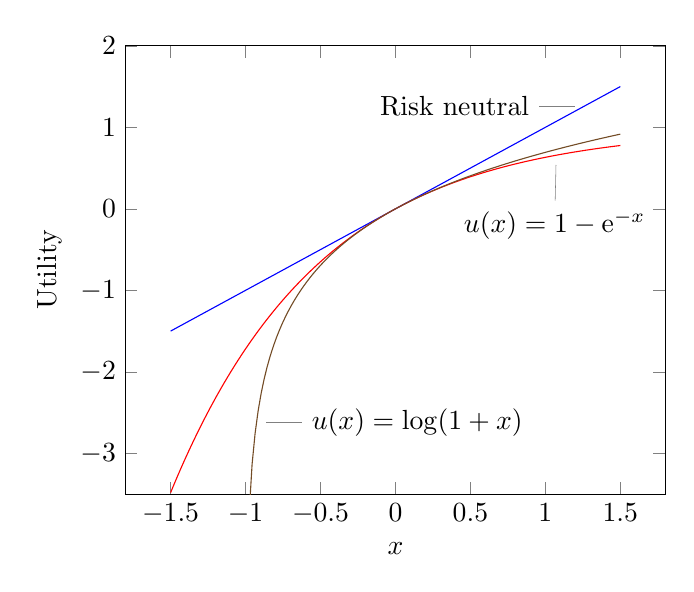
\begin{tikzpicture}
      \begin{axis}[
        xlabel=$x$,
        ylabel=Utility,
        domain=-1.5:1.5,
        samples=150,
        ymin=-3.5
        ]
        \addplot+[mark=none] {x}
        node[pos=0.92, pin={[black]180:Risk neutral}]{};
        \addplot+[mark=none] {1-exp(-x)}
        node[pos=0.92, pin={[black]-92:$u(x)=1-\mathrm{e}^{-x}$}] {};
        \addplot+[mark=none] {ln(1+x)}
        node[pos=0.4, pin={[black]0:$u(x)=\log(1+x)$}] {};
      \end{axis}
    \end{tikzpicture}
    \caption{Comparison of the exponential and logarithmic
      utilities. As $x$ approaches -1 from above, the utility to a logarithmic
      decision maker is modelled to be infinitely bad.
    }\label{fig:example_utilities}
  \end{figure}
\end{example}

For a given utility function that models a decision maker's measure of
benefit for the outcomes of $f$, one can formulate a well-defined
optimisation problem.

\begin{problem}[Expected utility]
  The optimal choice to maximise a given utility of $f$ is the
  solution of
  \begin{align}
    x(u)=\argmax_{x\in\mathcal{X}} \mathbb E[u(f(x,\cdot))].
  \end{align}
\end{problem}


\subsection{Mean-deviation problems}
The expected utility approach considers the mean outcome of a choice.
After one makes a decision $x\in\mathcal{X}$, the realisation of the
parameter in $\mathcal{Y}$ only happens once. If there is a large
uncertainty in $f(x,\cdot)$, the average value may not be a good
representation for the realised value of $f$.
It can therefore be useful to take into account some measure of
deviation from the mean of $f$ when $x$ is chosen.
The mean-deviation approach aims to balance the expected value of $f$
with uncertainty represented by a deviation measure.
\begin{mydef}[Deviation measure]
  A functional $\mathbb D$ on a linear space of random
  variables containing the real numbers defines a deviation measure, if:
  \begin{enumerate}
  \item $\mathbb D[C] = 0$ for any constant $C$,
  \item $\mathbb D[X]>0$ for non-constant random variables $X$.
  \end{enumerate}
  This work will mainly consider convex deviation measures.
\end{mydef}

\begin{example}[Deviation measures]
  The classic measure of deviation is the standard deviation, which is
  a particular case of the deviation measures defined by
  the $L^p$-norms:
  \begin{align}
    X\mapsto \|X-\mathbb EX\|_p,\; p\geq 1.
    && \text{($L^p$-deviations)}
  \end{align}

  In a maximisation setting, one might not be worried about
  realisations of $f$ that are larger than its mean, especially if the
  random variable is not symmetric.
  The lower semi-deviation measure only investigates
  worse-than-expected outcomes:
  \begin{align}
    X\mapsto \mathbb E[\max(\mathbb E[X]-X,0)].
    &&\text{(Lower semi-deviation)}
  \end{align}

  One can also combine two deviation-measures in order to capture
  different aspects of a random variable.
  If $\mathbb D_1,\dots,\mathbb D_k$ are $k$ deviation measures and
  $\lambda_i>0$, then the following is also
  is also a deviation measure:
  \begin{align}
    \mathbb D[X]=\sum_{i=1}^k\lambda_i\mathbb D[X].
    &&\text{(Weighted deviations)}
  \end{align}

  If $\mathbb U$ is a nonlinear expectation from
  \Cref{sec:nonlinear_expectations} with $\mathbb U[X]< \mathbb
  E[X]$ for all non-constant $X$,
  then one can
  construct a deviation measure with the functional
  $\mathbb D[X]=\mathbb E[X]-\mathbb U[X]$.
  This is equal to $X\mapsto -\mathbb U[X-\mathbb E[X]]$ in all the
  examples given below.
\end{example}

For a given deviation measure that models the decision maker's
need for stability, one can formulate a bi-objective optimisation
problem.
\begin{problem}[Mean-deviation]
  An optimal decision that maximises the expected value of $f$ whilst
  minimising the deviation $\mathbb D$ of $f$, is a minimiser to the
  bi-objective optimisation problem
  \begin{align}
    \min_{x\in\mathcal{X}}\{(\mathbb E[f(x,\cdot)],-\mathbb D[f(x,\cdot)])\}.
  \end{align}
\end{problem}
The bi-objective problem can be approached from a multiobjective
optimisation theory point of view.
The review in \citep{marler2004survey} covers some of the theory,
discusses what optimality means and introduces approaches to solve them.
A simple approach is to define a single objective function that combines
the expected value with a deviation-penalty, weighted by some
parameter $\lambda>0$. The optimal decision in $\mathcal{X}$ is then
defined as
\begin{align}
  x(\mathbb D,\lambda)=\argmax_{x\in\mathcal{X}}\{\mathbb
  E[f(x,\cdot)]-\lambda \mathbb D[f(x,\cdot)]\}.
\end{align}
If $f$ is nonlinear, then $x(\mathbb D,\lambda)$ can be unstable to
small changes in $\lambda$. So small errors in determining the best
$\lambda$ to represent a decision-maker can cause large changes in
either of the objectives. More robust methods are covered in
\citep{marler2004survey}.

\subsection{Nonlinear expectations}\label{sec:nonlinear_expectations}
A general framework that covers most of the remaining
in optimisation under uncertainty makes use of a class of functionals
called nonlinear expectations.
The theory was developed in finance to study financial positions using
risk measures, see
e.g.~\citep[Ch.~4]{follmer2004stochastic}.
Risk measures are used in a minimisation setting related to losses,
and we will use the term nonlinear expectations in the maximisation
setting. The examples of nonlinear expectations $\mathbb U$ considered
in this section give rise to well-known risk measures $\rho$, by using the mapping
$\rho(X) = -\mathbb U[X]$.

\begin{mydef}[Nonlinear expectation]
  A nonlinear expectation $\mathbb U$ is a functional on a linear space of random
  variables containing the real numbers, such that:
  \begin{enumerate}
  \item $\mathbb U[C] = C$ for any constant $C$,
  \item $\mathbb U[X]\leq \mathbb U[Y]$ whenever $X\leq Y$ almost surely.
  \end{enumerate}
  This work will mainly consider concave nonlinear expectations, that
  is, nonlinear expectations $\mathbb{U}$ such that
  $\mathbb{U}[\lambda X + (1-\lambda)Y]\geq \lambda\mathbb{U}[X] +
  (1-\lambda) \mathbb{U}[Y]$ for any $\lambda\in[0,1]$ and random
  variables $X,Y$.
\end{mydef}

\begin{example}[Nonlinear expectations]
  The functional $\mathbb U_\lambda[X]=-\frac{1}{\lambda}\log\mathbb
  E[\mathrm{e}^{-\lambda X}]$, is called the entropic nonlinear expectation,
  with $\lambda>0$.
  It is connected to the exponential utility function $u_\lambda$, since
  $\mathbb U_\lambda[X]= u_\lambda^{-1}(\mathbb E[u_\lambda(X)])$.

  The worst-case nonlinear expectation on the sample space $\Omega$,
  defined by
  $X\mapsto  \inf_{\omega\in\Omega}X(\omega)$, connects this theory with robust
  programming. If there is an attached probability space on $\Omega$,
  we use the essential infimum.

  For some deviation measures $\mathbb D$, like the lower
  semi-deviation, the functional $\mathbb U(X)=\mathbb E[X]-\mathbb
  D[X]$ defines a nonlinear expectation. Note that for a general space
  of random variables the symmetric deviation measure, like the
  standard deviation, do not give rise to a nonlinear
  expectation: They can violate the monotonicity requirement.

  The quantile operator
  $q_\lambda[X] = \inf\{x\mid\mathbb P(X\leq x)>
  \lambda\}$ satisfies the properties of a nonlinear expectation.
  In an optimisation setting, it is important to note that it is not
  necessarily concave.
  A concave lower bound on the quantile operator is
  the negative of the \emph{Average Value at Risk} measure:
  \begin{align}
    \mathbb U_\lambda[X]=\frac{1}{\lambda}\int_0^\lambda q_t[X]\,\dt.
  \end{align}
\end{example}

\begin{problem}[Nonlinear expectation]
  The optimal choice to maximise a nonlinear expectation
  of $f$ is given by
  \begin{align}
    x(\mathbb U)=\argmax_{x\in\mathcal{X}} \mathbb U[f(x,\cdot)].
  \end{align}
\end{problem}

\emph{Remark:} The solutions of the nonlinear expectation and expected
utility problems coincide if one uses the entropic measure and the exponential
utility respectively.

\subsection{Randomness and constraints}
Let us introduce another, deterministic, objective $g:\mathcal
X\to\mathbb R$. In the deterministic setting, where
the parameter $y\in\mathcal{Y}$ is known, one often considers problems
of the form
\begin{align}
  \min_{x\in\mathcal{X}}\{g(x)\mid f(x,y)\geq f_{min} \},\;
  \text{ for some } f_{min}\in\mathbb R.
\end{align}
Then $f\geq f_{min}$ is considered a constraint, which restricts the
decision space to $\{x\in\mathcal{X}\mid f(x,y)\geq f_{min}\}$.
When there is uncertainty about the right parameter-value, this set is
not defined at the time of decision, but depends on the realisation of
the parameter.

In the engineering community it is popular to
reinterpret non-deterministic ``constraints'' as deterministic via
expected utilities, mean-deviation methods or nonlinear
expectations~\cite{tyrrell2015engineering}.
This approach treats what was previously considered a hard constraint
in terms of marginalised values that allow decisions $x\in\mathcal{X}$
that can violate the original constraint for some values of the random
variable $y$. We argue that a better approach is to take one step back
and model the trade-off between $g(x)$ and the outcomes of $f(x,y)$.

\todo[inline]{Consider adding the example I had in my transfer}
We will solve such problems by combining the functions $g$ and $f$ to
a new objective. For example, we can attach a total utility to $g$ and
$f$, which takes into account potential tradeoffs between maximising
the two objectives. This includes penalty-type multivariate utilities
such as $U(g,f)=g-\max(f_{min}-f,0)$.


\section{Multiobjective optimisation}\label{sec:one_multiobjective}
\begin{itemize}
\item Copy stuff from transfer thesis
\item Include (and update) MultiJuMP example
\item Show example of mean-std with revenue: Pareto is not convex
\end{itemize}

\section{Comparison of ordering methods for random outcomes}\label{sec:one_comparison_orderings}



\biblio{} % Bibliography when standalone
\end{document}

%%% Local Variables:
%%% mode: latex
%%% TeX-master: t
%%% TeX-command-extra-options: "--shell-escape"
%%% TeX-command-extra-options: "-shell-escape"
%%% End:
